\chapter{Part I(b) - ISA, Functions, and Stack - W 1.2}
\section{Arithmetic and Logic Instructions in RISCV}
\textit{Bellow some examples of RISCV instructions:} \\
\textbf{Two Operands Instructions} \\
\vspace*{10px}
\begin{minipage}{0.4\textwidth}
\begin{assembly}
sll  x5, x5, x9
add  x6, x5, x7
xor  x6, x6, x8
slt  x8, x6, x7
\end{assembly}
\end{minipage}%
\hfill
\vline
\hfill
\begin{minipage}{0.5\textwidth}
\small
\textit{Shift x5 left by x9 positions $\rightarrow$ x5} \\
\textit{Add x5 and x7 $\rightarrow$ x6} \\
\textit{Logic XOR bitwise x6 and x8 $\rightarrow$ x6} \\
\textit{Set x8 to 1 if x6 is lower than x7, otherwise to 0}
\end{minipage}

\textbf{Arithmetic Instructions} \\
\vspace*{10px}
\begin{minipage}{0.4\textwidth}
\begin{assembly}
slli x5, x5, 3
addi x6, x5, 72
xori x6, x6, -1
slti x8, x6, 321
\end{assembly}
\end{minipage}%
\hfill
\vline
\hfill
\begin{minipage}{0.5\textwidth}
\small
\textit{Shift x5 left of 3 positions $\rightarrow$ x5} \\
\textit{Add 72 to x5 $\rightarrow$ x6} \\
\textit{Logic XOR bitwise x6 and 0xFFFFFFFF $\rightarrow$ x6} \\
\textit{Set x8 to 1 if x6 is lower than 321, to 0 otherwise} \\
\end{minipage} \\
\textbf{Here, you may ask yourself, why are all immediates (constants) writtent on a maximum of 12bits?} \\
\subsection{Constants must be encoded on 12 bits}
\textit{As you may see here, all instructions encode immediates on 12 bits.}
\begin{center}
    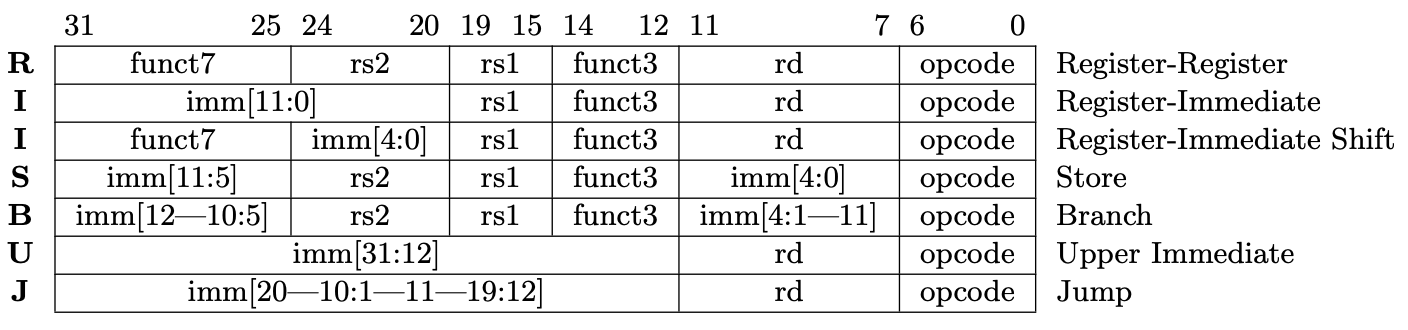
\includegraphics[width=0.8\textwidth]{chapters/chapter1b/images/riscv.png}
\end{center}

\subsection{Assembler Directives} \textit{Assembler directives help write cleaner and more readable code. The code snippets on the left and right below are equivalent.}

\begin{center} 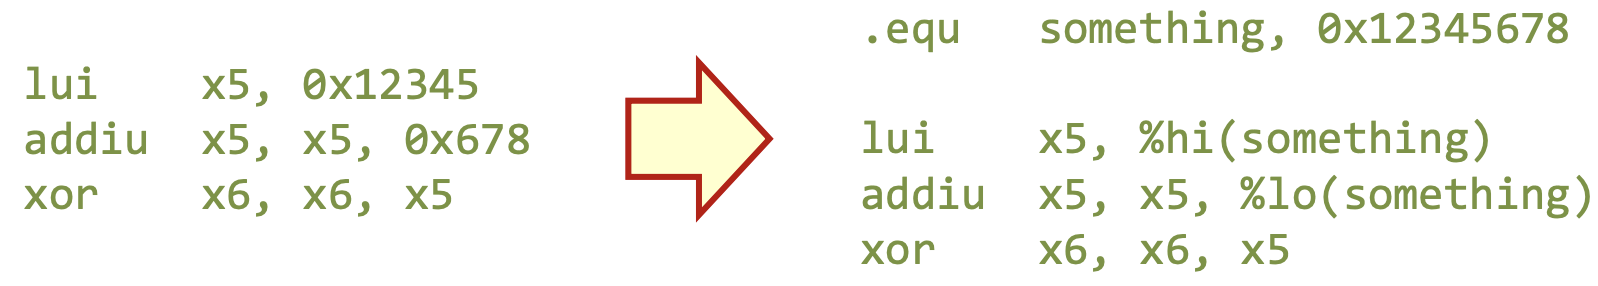
\includegraphics[width=0.65\textwidth]{chapters/chapter1b/images/directives.png} \end{center}

The left-hand side code snippet shows an assembly sequence where a 32-bit constant value (\texttt{0x12345678}) is loaded into a register (\texttt{x5}). Since immediate values are 16-bit limited, this requires splitting the 32-bit value into two instructions: 

\begin{itemize}
    \item[-] The first instruction, \texttt{lui}, loads the upper 16 bits (\texttt{0x12345}) into the register \texttt{x5}.
    \item[-] The second instruction, \texttt{addiu}, adds the lower 16 bits (\texttt{0x678}) to \texttt{x5}, completing the full 32-bit value in the register.
\end{itemize}

\textit{This approach, while functional, can become cumbersome when dealing with multiple constants, making the code less readable and harder to maintain. \\
} 
\vspace*{5px}
The right-hand side shows the same functionality but makes use of assembler directives, specifically the \texttt{.equ} directive to define a label (\texttt{something}) for the constant \texttt{0x12345678}. Using the \texttt{\%hi()} and \texttt{\%lo()} pseudo-instructions, the assembler automatically splits the constant into its upper and lower parts:

\begin{itemize}
    \item[-] The \texttt{\%hi(something)} loads the upper 16 bits into \texttt{x5}.
    \item[-] The \texttt{\%lo(something)} adds the lower 16 bits to \texttt{x5}.
\end{itemize}

This method enhances code clarity and maintainability, especially when working with multiple constants, by using human-readable labels instead of raw numeric values. The assembler handles the details of splitting the 32-bit constant into its upper and lower parts.
\begin{center} 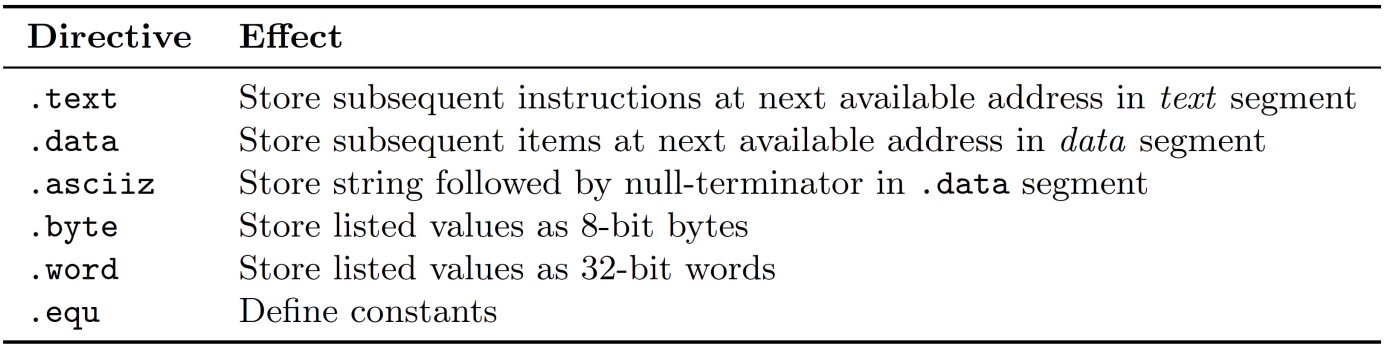
\includegraphics[width=0.65\textwidth]{chapters/chapter1b/images/directives2.png} \end{center}

\subsection{The \texttt{x0} Register} 
\textit{The \texttt{x0} register is hardwired to 0 and cannot be changed.} \ \textit{Any attempt to write into \texttt{x0} will have no effect.}

\texttt{Why is this useful?} \\
One common application is in introducing wait delays during program execution. By leveraging the fixed nature of \texttt{x0}, it simplifies certain instructions that require an immediate zero value.

\section{PseudoInstructions}
\textit{PseudoInstructions simplify commands involving the \texttt{x0} register by creating easier-to-use alternatives.} \newline
\begin{center}
        \begin{tabular}{|c|c|c|}
        \hline
        \textbf{Pseudoinstruction} & \textbf{Base Instruction(s)} & \textbf{Meaning} \\ \hline
        \texttt{nop}               & \texttt{addi x0, x0, 0}      & No operation     \\ \hline
        \texttt{li rd, immediate}  & Myriad sequences             & Load immediate   \\ \hline
        \texttt{mv rd, rs}         & Myriad sequences             & Copy register    \\ \hline
        \texttt{not rd, rs}        & \texttt{xori rd, rs, -1}     & One's complement \\ \hline
        \texttt{neg rd, rs}        & \texttt{sub rd, x0, rs}      & Two's complement \\ \hline
        \texttt{seqz rd, rs}       & \texttt{sltiu rd, rs, 1}     & Set if = zero    \\ \hline
        \texttt{snez rd, rs}       & \texttt{sltu rd, x0, rs}     & Set if $\neq$ zero    \\ \hline
        \texttt{sltz rd, rs}       & \texttt{slt rd, rs, x0}      & Set if < zero    \\ \hline
        \texttt{sgtz rd, rs}       & \texttt{slt rd, x0, rs}      & Set if > zero    \\ \hline
        \end{tabular}
\end{center} 
The term \textit{myriad sequences} refers to a series of instructions that together achieve the functionality of a single pseudoinstruction, such as using \texttt{lui} and \texttt{addi} to implement \texttt{li rd, immediate}.

\textbf{According to the professor li should be called \texttt{mvi} (as move immediate).}

\subsection{Control flow instructions}
\textit{Control flow instructions are used to change the order of execution of instructions are a kind of pseudo-instructions.}
\begin{assembly}
    li x1, 0x00123456
    li x2, 0
    li x3, 1
    li x4, 0
    li x5, 0
    li x6, 32
loop: and x5, x1, x3
    add x2, x2, x5
    srli x1, x1, 1
    addi x4, x4, 1
    bne x4, x6, loop
\end{assembly}

\subsection{If-Then-Else}
\begin{minipage}[htp]{0.4\textwidth}
\begin{cc}
if (x5 == 72) {
    x6 = x6 + 1;
    } else {
    x6 = x6 - 1;
}
\end{cc}    
\end{minipage}
\hfill
\vline
\hfill
\begin{minipage}[htp]{0.4\textwidth}
\begin{assembly}
.text
    li x7, 72
    beq x5, x7, then_clause
else_clause:
    addi x6, x6, -1
    j end_if
then_clause:
    addi x6, x6, 1
end_if:
\end{assembly}
\end{minipage} \\
\vspace*{5px}
\textit{As seen here, beqi does not exist in RISCV, instead we use \texttt{beq} and \texttt{li} to achieve the same result.}
\subsection{Jumps and Branches}
A common but not universal distinction exists between \emph{jumps} and \emph{branches}. In RISC-V (inherited from MIPS and used by SPARC, Alpha, etc.), jumps refer to unconditional control transfer instructions, while branches refer to conditional control transfer instructions. However, not all architectures follow this convention. For instance, in x86, all control transfer instructions are considered jumps, such as \texttt{JMP}, \texttt{JZ}, \texttt{JC}, and \texttt{JNO}.

\subsection{Comparaisions}
\textit{The processor implements only $<$ and $>$, and the assembler “creates” $\leq$ and $\geq$.}

\begin{center}
    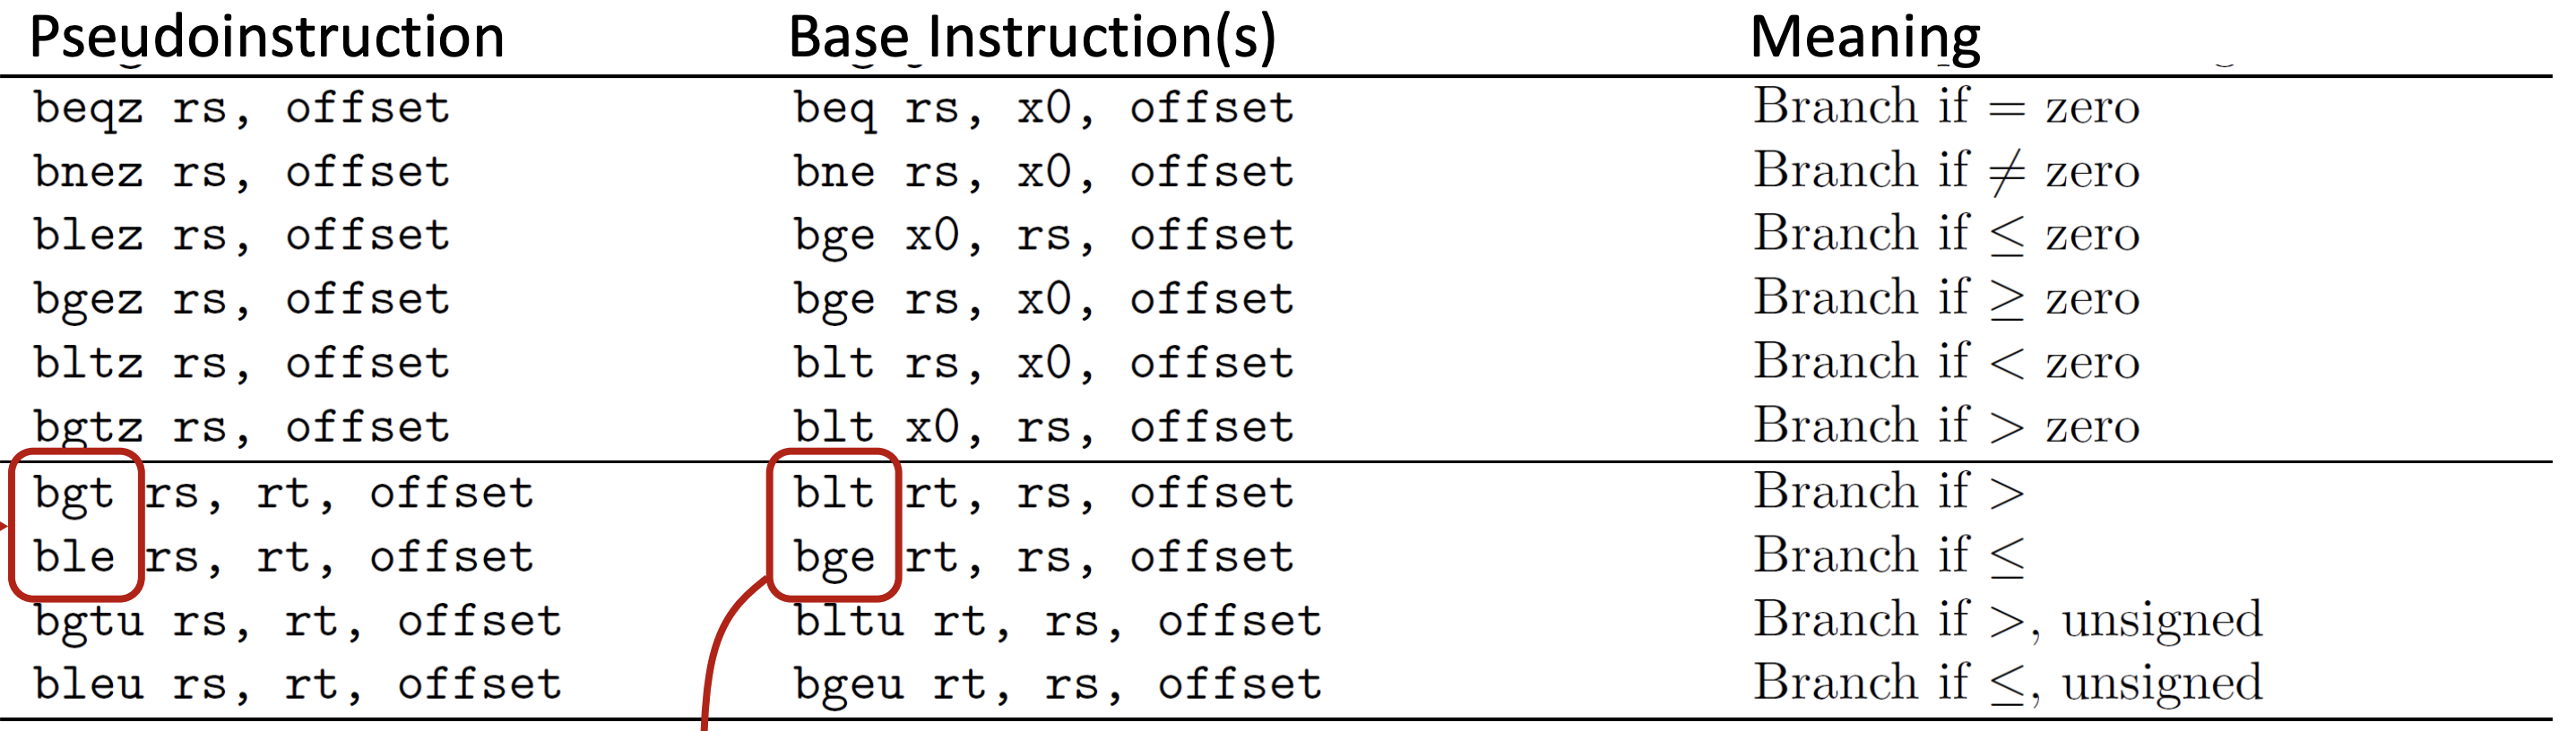
\includegraphics[width=0.75\textwidth]{chapters/chapter1b/images/comp.png}
\end{center}
\subsection{Do-While}
\textit{Do-while loops look like this (we obviously use control flow instructions here).} \\
\begin{minipage}[htp]{0.4\textwidth}
\begin{cc}
do {
    x5 = x5 >> 1;
    x6 = x6 + 1;
} while (x5 != 0);
\end{cc}    
\end{minipage}
\hfill
\vline
\hfill
\begin{minipage}[htp]{0.4\textwidth}
\begin{assembly}
.text
loop:
    srli x5, x5, 1
    addi x6, x6, 1
    bnez x5, loop
\end{assembly}
\end{minipage}

\section{Functions}
\textit{In higher-level programming languages, functions (routines, subroutines, procedures, methods, etc.) are used to encapsulate code and make it reusable. } \\
\textbf{Calling a function involves these steps:}
\begin{enumerate}
    \item Place arguments where the called function can access them.
    \item Jump to the function.
    \item Acquire storage resources the function needs.
    \item Perform the desired task of the function.
    \item Communicate the result value back to the calling program.
    \item Release any local storage resources.
    \item Return control to the calling program.
\end{enumerate}
\subsection{Jump to the Function/Retun control to the calling program}
\subsubsection{The too simple not working approach}
A simple (not working) approach for creating functions would be to do this: 
\begin{center}
    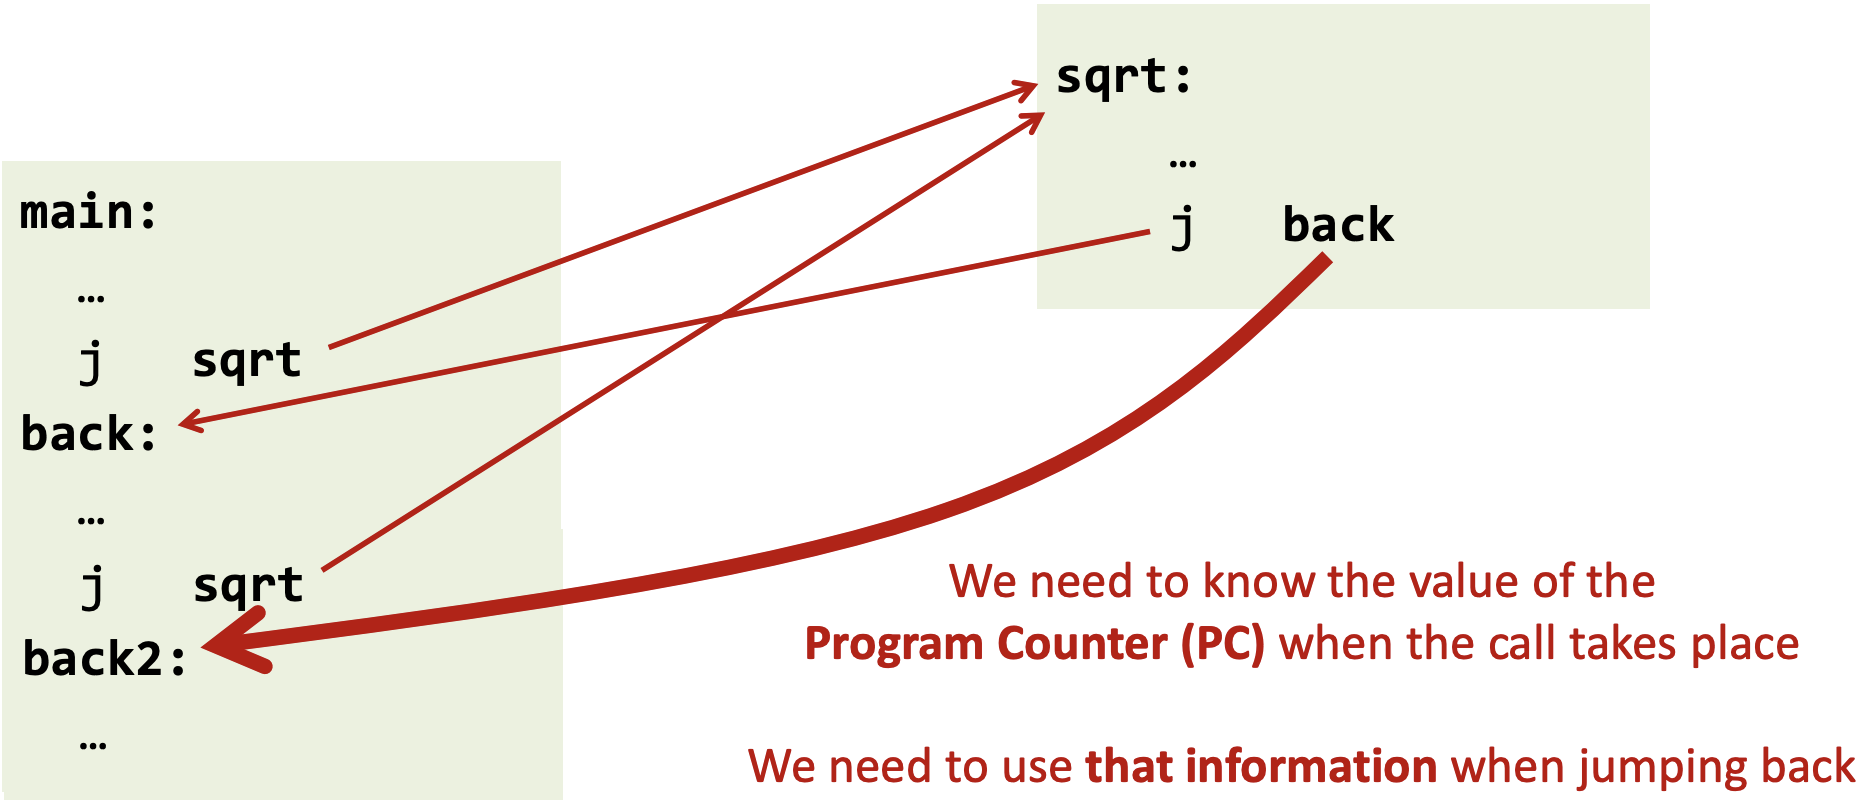
\includegraphics[width=0.75\textwidth]{chapters/chapter1b/images/function.png}
\end{center}
\textit{With this approach the function doesn't know where to return to after being called (back2 or back)}
\textbf{For the next part, remember, the Program Counter is distinct from general-purpose registers. It is dedicated to managing the flow of instruction execution, while general registers are used for data manipulation. }
\subsubsection{The Good Approach}
\textit{The right approach involves using the Jump and Link instruction \texttt{jal}, here loading PC + 4 (remember 4 bytes per Instruction) into x1 as a way to come back from the function.} \\
\begin{minipage}[htp]{0.4\textwidth}
\begin{assembly}
main:
    ...
    jal x1, sqrt
    ...
    ...
    jal x1, sqrt
\end{assembly}    
\end{minipage}
\hfill
\vline
\hfill
\begin{minipage}[htp]{0.4\textwidth}
\begin{assembly}
sqrt:
    ...
    ...
    jr x1
\end{assembly}
\end{minipage} \\
\textit{Both times x1 was used to store the return adress, and there is a reason for that (Register Conventions Sections).}

\subsection{Jump Instructions}
\textit{There are only two core real jump instructions in RISCV, \texttt{jal} (jump and link) and \texttt{jalr} (jump and link register), the rest are pseudo instructions using them.} \\

\begin{center}
    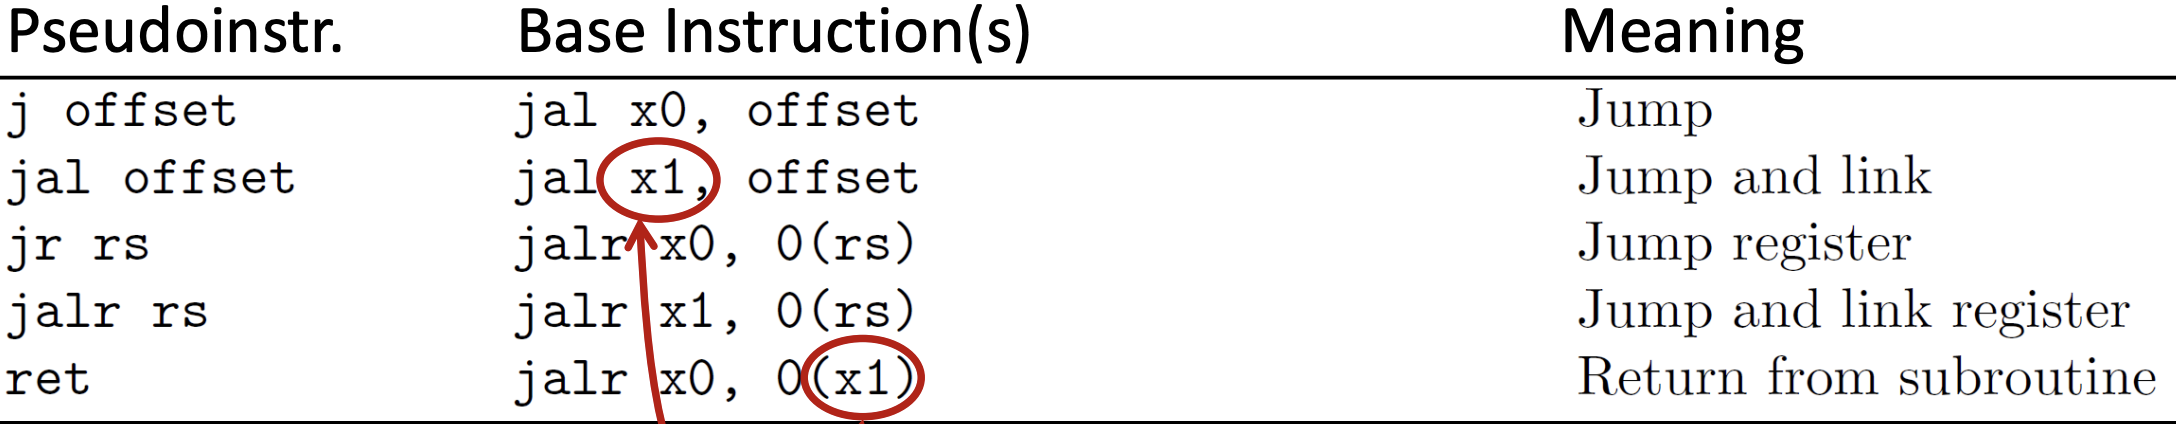
\includegraphics[width=0.75\textwidth]{chapters/chapter1b/images/jump.png}
\end{center}
\newpage
\subsection{Register Conventions}
\textit{Register conventions are rules that dictate how registers are used in a program, here are the ones we've seen for now} \\
\begin{center}
    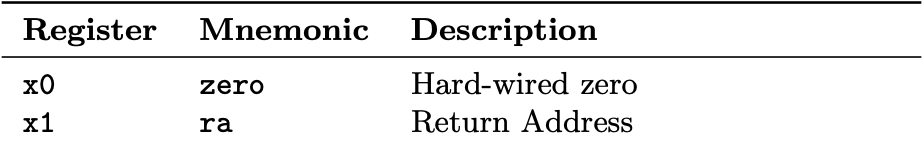
\includegraphics[width=0.75\textwidth]{chapters/chapter1b/images/conventions.png}
\end{center}

\subsection{Back to the good (not so good) approach}
\textit{There's still a problem with the previous approach, say for example you want to call a function from another function.}
\begin{center}
    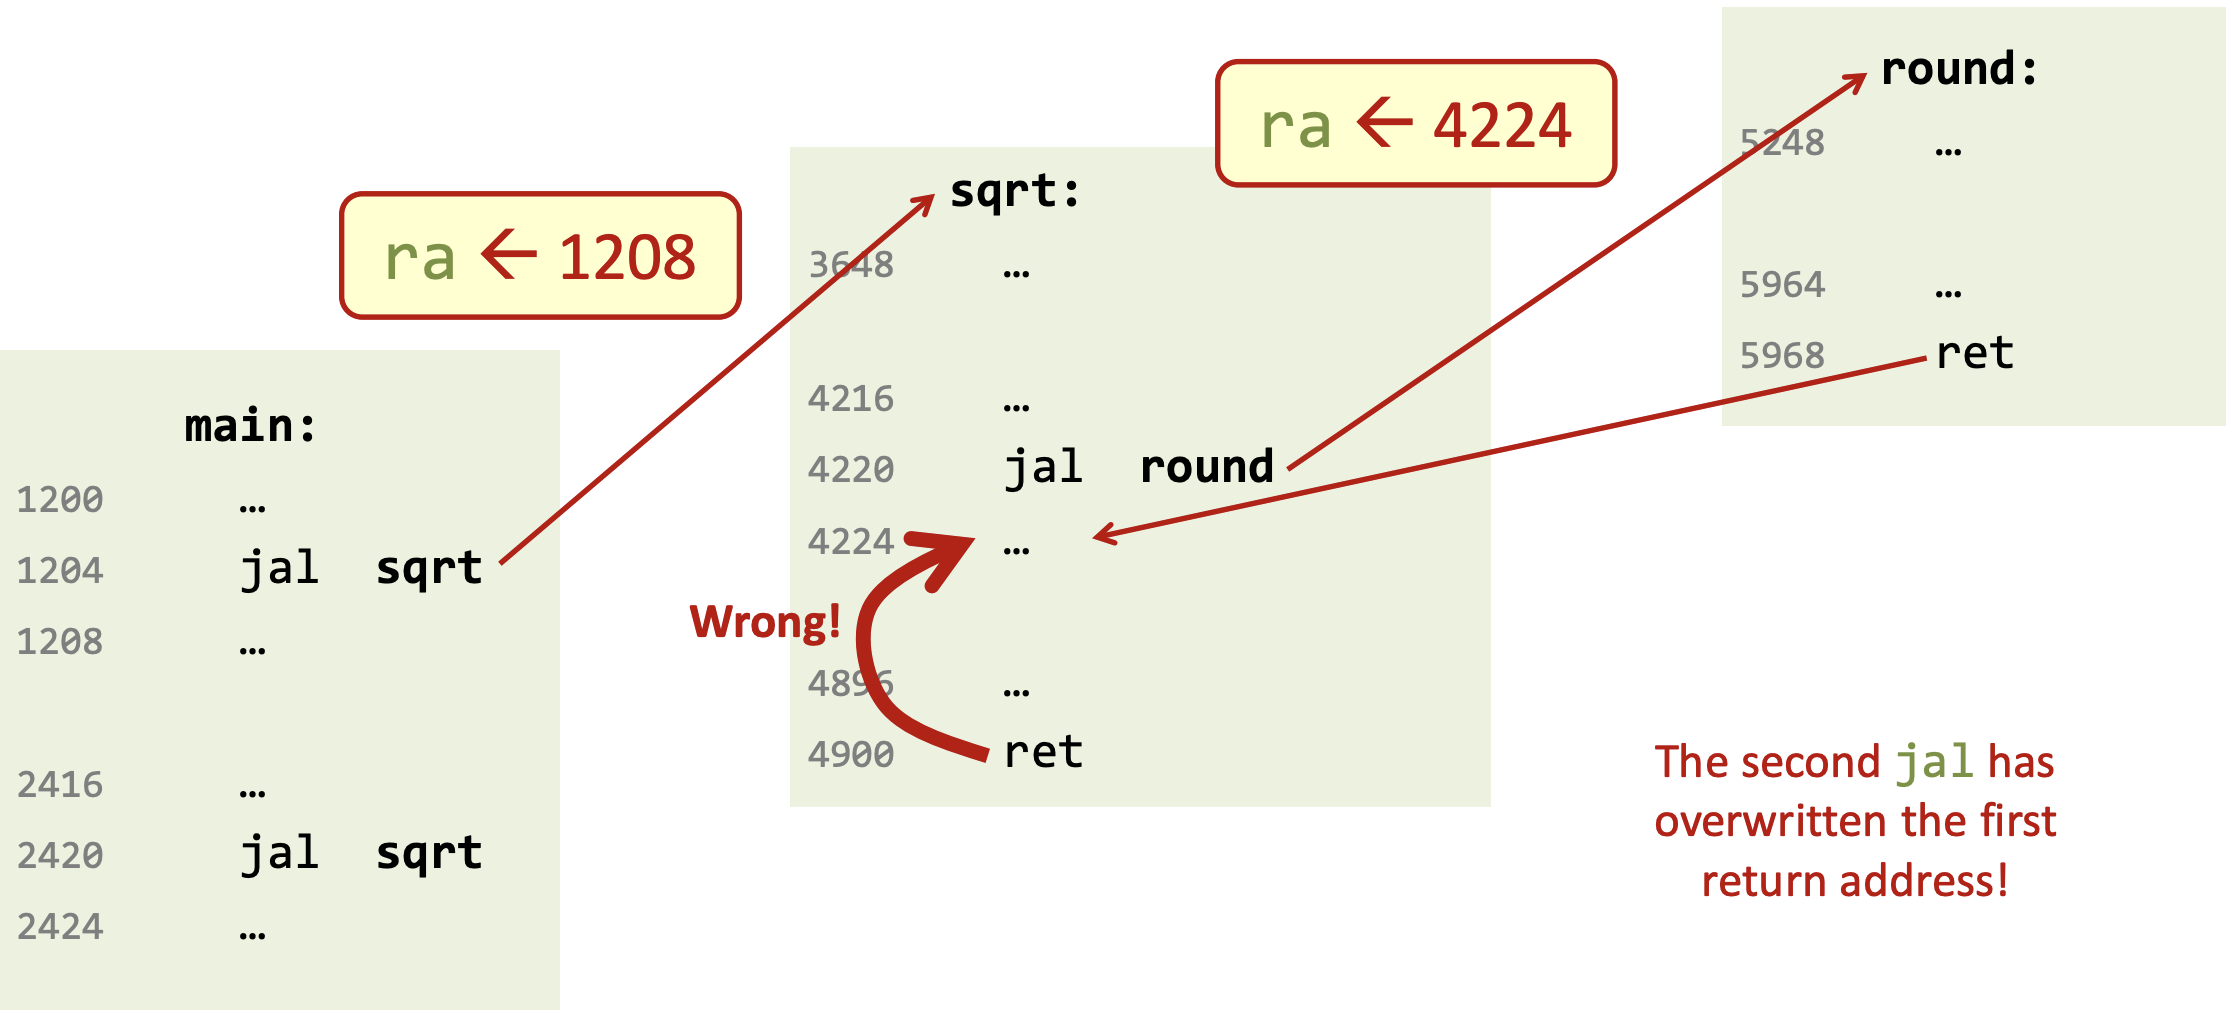
\includegraphics[width=0.75\textwidth]{chapters/chapter1b/images/function2.png}
\end{center}
\textbf{Here the allocated space for the return address is overwritten by the second function call, and the first function can't return to the right place.}
\subsection{One simple solution (still not good)}
\textit{One solution would be to say that a range of registers are used for certain functions and that they can't be used by other functions.}
\begin{center}
    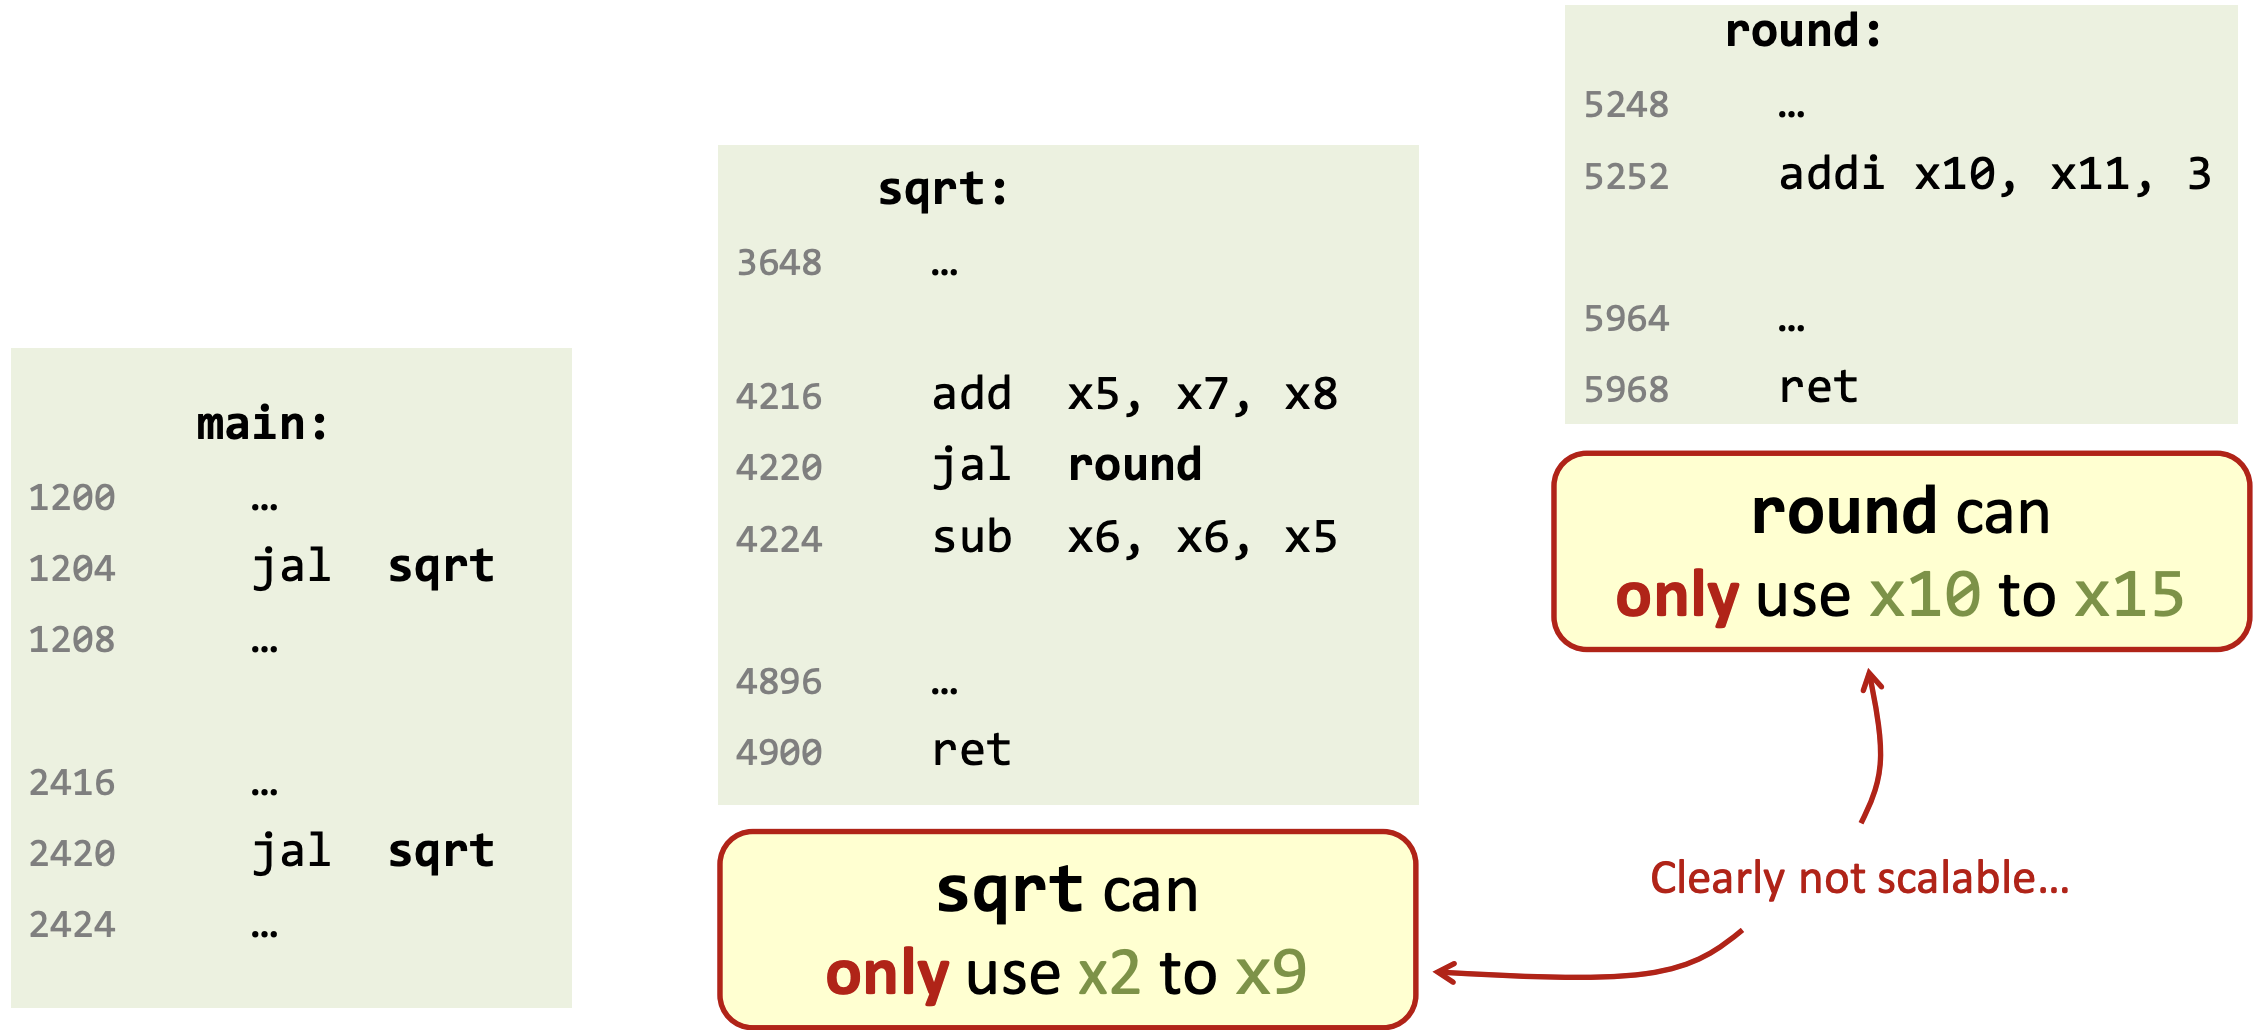
\includegraphics[width=0.75\textwidth]{chapters/chapter1b/images/function3.png}
\end{center}
\textbf{The problem here is that it's still not very scalable.}
\subsection{Acquire storage resources the function needs (still not it)}
One simple solution to our problem would be to allocate memory for the function at in the data section of the program. \\
\begin{minipage}[htp]{0.4\textwidth}
\begin{assembly}
.data
sqrt_save_ra: .word 0
sqrt_save_x5: .word 0 
\end{assembly}
\end{minipage}
\hfill
\vline
\hfill
\begin{minipage}[htp]{0.4\textwidth}
\begin{assembly}
.text
sqrt:
...
add x5, x7, x8
sw ra, sqrt_save_ra
sw x5, sqrt_save_x5
jal round
lw ra, sqrt_save_ra
lw x5, sqrt_save_x5
sub x6, x6, x5
...
ret
\end{assembly}
\end{minipage}
\subsubsection{Problem: Recursive Functions}
\textit{The problem here is that the return address is overwritten by the recursive call.}
\begin{center}
\begin{assembly}
.data
    find_child_save_ra: .word 0
.text
    find_child:
    ...
    sw ra, find_child_save_ra
    jal find_child
    lw ra, find_child_save_ra
    ...
    ret
\end{assembly}
\end{center}
\subsection{The Stack}
\textit{The Solution to our Problem is this, the Stack.} \\
\textbf{The Stack is a region of memory that grows and shrinks as needed.} \\
We may use a register (e.g \texttt{x2}) to point to the first used word after the end of the used region.
\begin{center}
    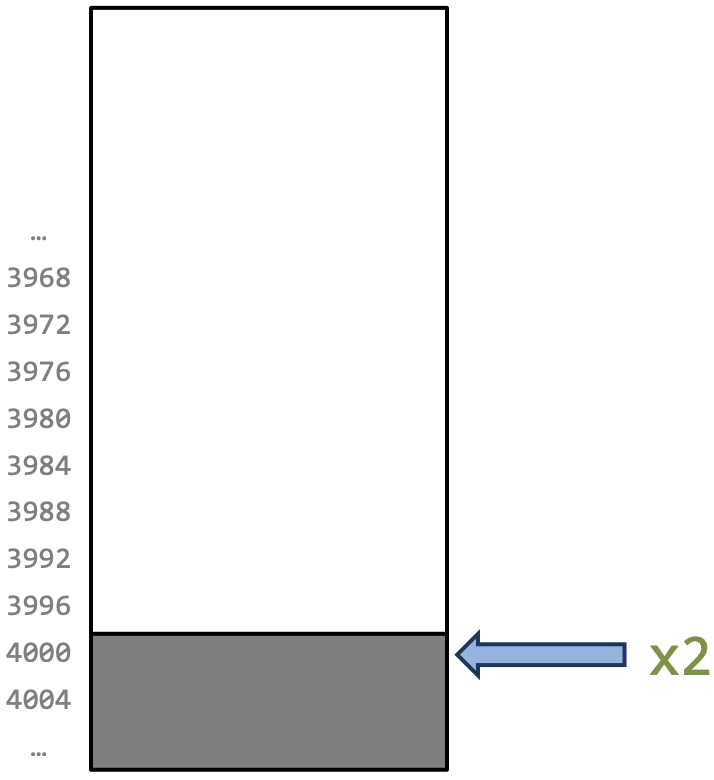
\includegraphics[width=0.4\textwidth]{chapters/chapter1b/images/stack.png}
\end{center}

\subsubsection{Dynamic Memory Allocation}
The Stack, contrary to the Data Section, is dynamic and can be used to allocate memory when needed. This means that during program execution, variables or temporary data can be stored in the stack, which grows or shrinks depending on the operations performed. \\
 The \texttt{stack pointer}, typically register x2, is used to manage the allocation and deallocation of memory.

\begin{minipage}[htp]{0.4\textwidth}
\textit{In this instruction, for example, we allocate 12 bytes in the stack. We achieve this by decrementing the stack pointer (x2) by 12. This ensures that the new memory space is available for temporary storage.}
\begin{assembly}
addi x2, x2, -12
\end{assembly}
\end{minipage}
\hfill
\vline
\hfill
\begin{minipage}[htp]{0.4\textwidth}
\begin{center}
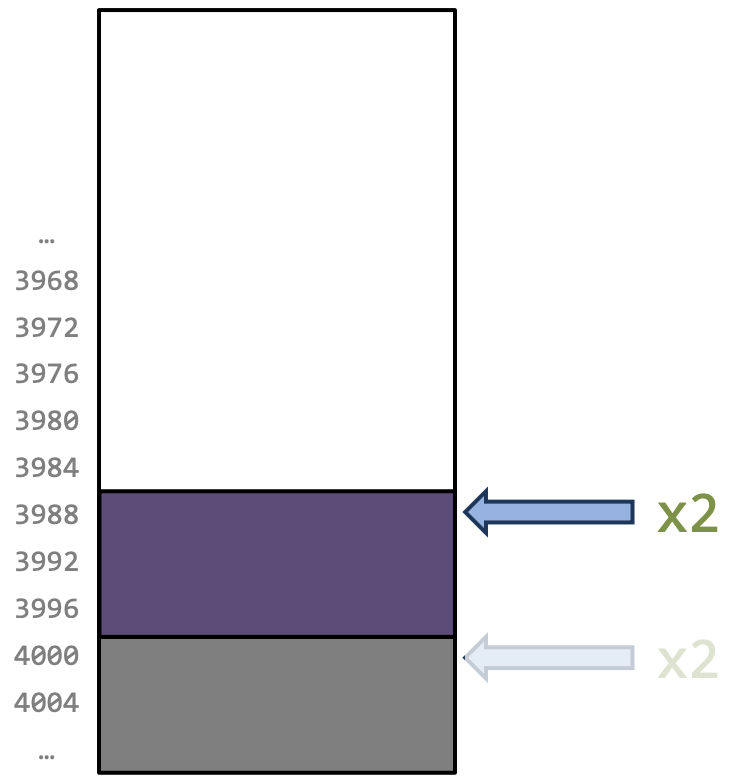
\includegraphics[width=0.75\textwidth]{chapters/chapter1b/images/stack2.png}
\end{center}
\end{minipage}

\subsubsection{Retrieving Data from the Stack}
Once memory has been allocated on the stack, we can store or retrieve data from it. In this case, we are retrieving data that was previously saved in the stack. The lw (load word) instruction is used to load the values stored at different offsets in the stack.

\begin{minipage}[htp]{0.4\textwidth}
\textit{In this case, we retrieve three different values from the stack using the lw instruction, which loads a 4-byte value into the specified registers (ra, x5, and x6). The offsets (0, 4, and 8) refer to different positions in the 12 bytes we allocated earlier.}
\begin{assembly}
lw ra, 0(x2)
lw x5, 4(x2)
lw x6, 8(x2)
\end{assembly}
\end{minipage}
\hfill
\vline
\hfill
\begin{minipage}[htp]{0.4\textwidth}
\begin{center}
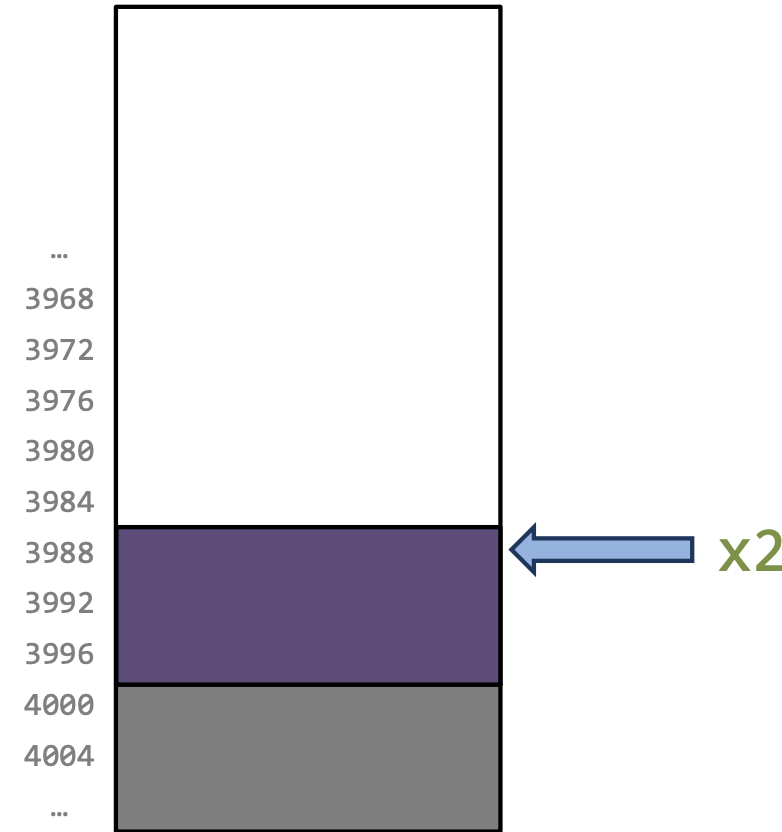
\includegraphics[width=0.75\textwidth]{chapters/chapter1b/images/stack3.png}
\end{center}
\end{minipage}
\newpage

\subsubsection{Memory Deallocation}
After the data has been used or is no longer needed, it is good practice to deallocate the memory to ensure proper management of the stack. We deallocate memory by adjusting the stack pointer (x2) back to its original position.

\begin{minipage}[htp]{0.4\textwidth}
\textit{In this instruction, we restore the stack to its previous state by adding 12 back to the stack pointer (x2).} \\ \textit{This effectively "frees" the 12 bytes of memory we had allocated earlier.}
\begin{assembly}
addi x2, x2, 12
\end{assembly}
\end{minipage}
\hfill
\vline
\hfill
\begin{minipage}[htp]{0.4\textwidth}
\begin{center}
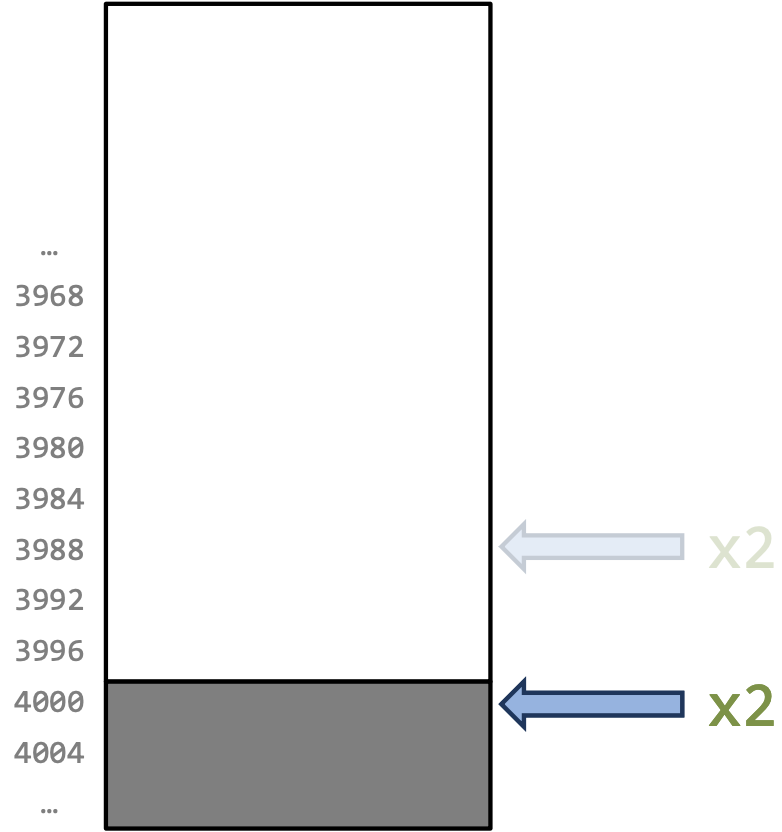
\includegraphics[width=0.75\textwidth]{chapters/chapter1b/images/stack4.png}
\end{center}
\end{minipage}

\subsubsection{The Stack Pointer}
\textit{The Stack Pointer is a register that points to the top of the stack, by convention it corresponds to the x2 register} \\
\begin{center}
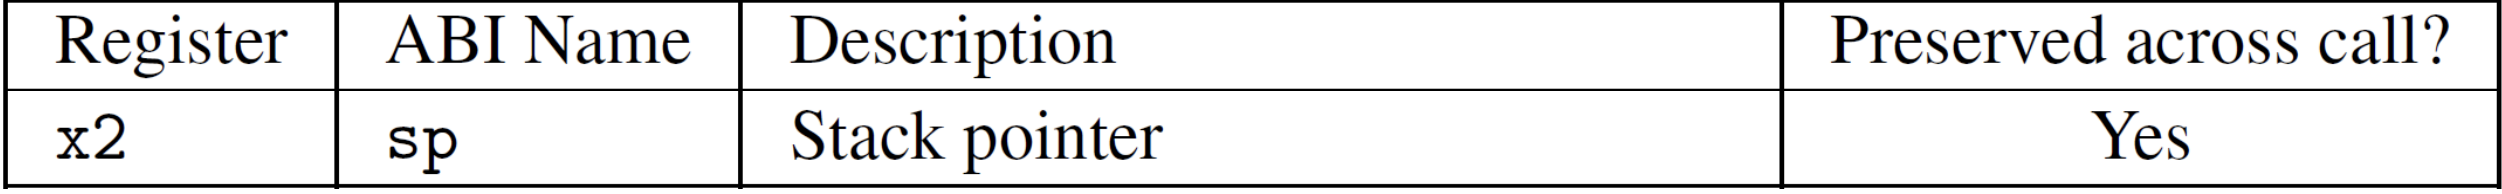
\includegraphics[width=0.75\textwidth]{chapters/chapter1b/images/conventions2.png}
\end{center}
\small
\textit{Other architectures have special instructions to place stuff on
the stack (push) and to retrieve it (pop)} \\
\vspace*{10px}
\begin{minipage}[htp]{0.4\textwidth}
\begin{lstlisting}
PUSH AX
\end{lstlisting}
\end{minipage}
\hfill
\vline
\hfill
\begin{minipage}[htp]{0.4\textwidth}
\begin{assembly}
add sp, sp, -4
sw x5, 0(sp)
\end{assembly}
\end{minipage}

\subsection{Spilling Registers to Memory}
\textit{Spilling registers to memory involves saving register values to the stack when more registers are needed or to prevent overwriting important data, allowing the registers to be reused. This technique is also used in function calls to save the return address, ensuring the program can correctly return control after the function finishes.}
\begin{center}
    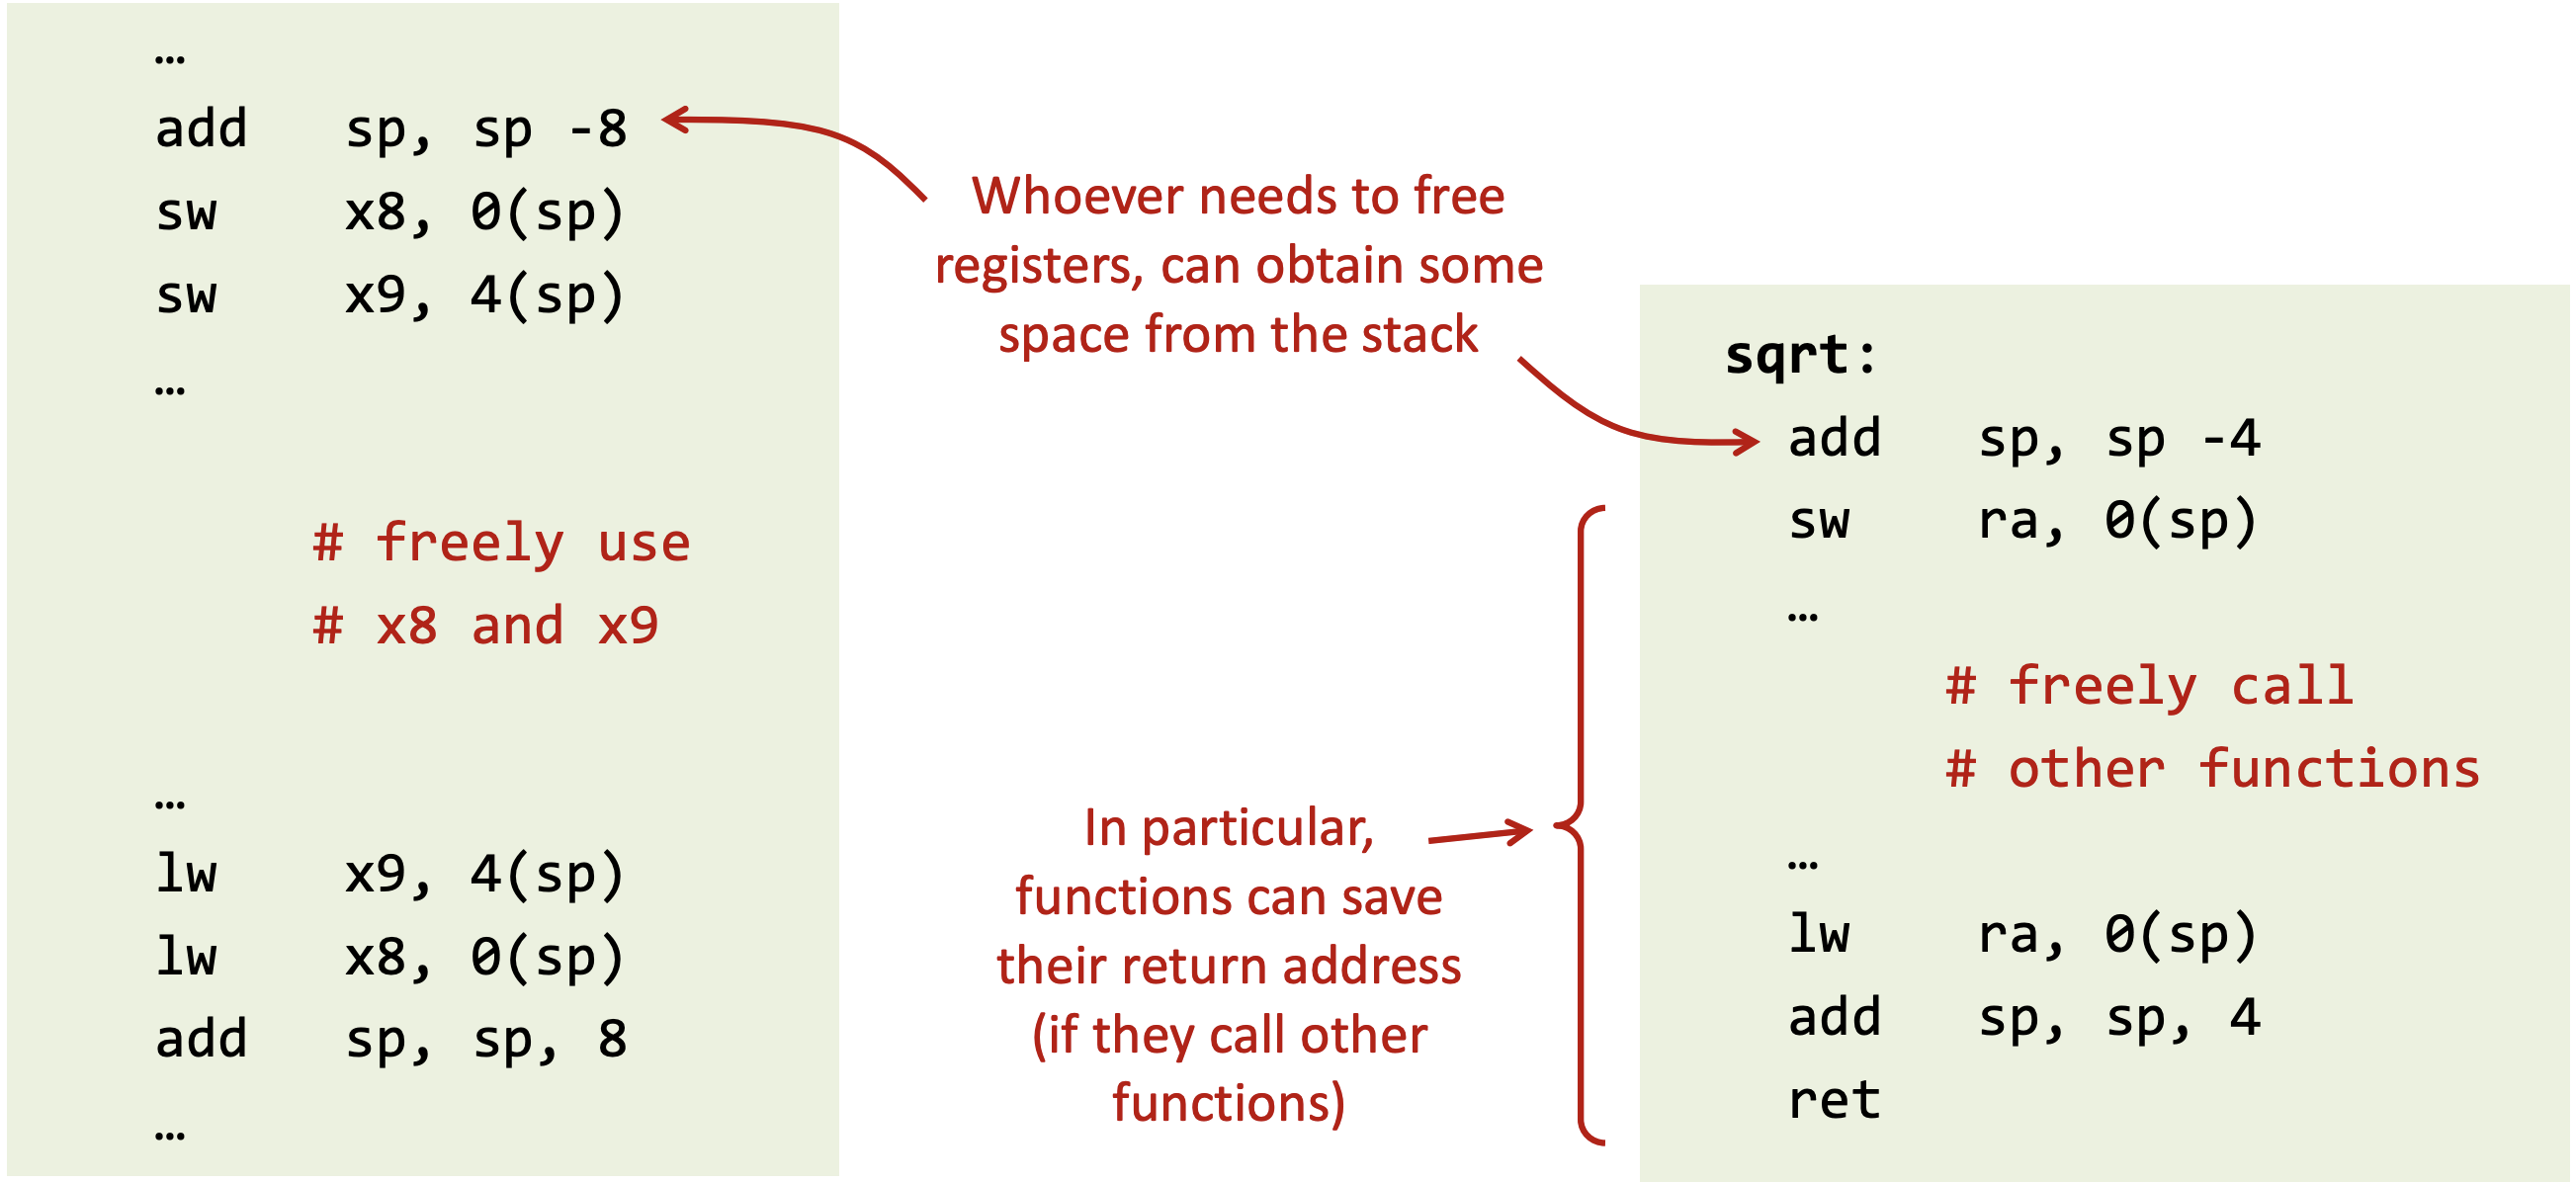
\includegraphics[width=0.75\textwidth]{chapters/chapter1b/images/spilling.png}
\end{center}

\subsection{Register across functions}
In assembly programming, handling registers across functions can be managed in two main ways: either functions \textbf{change registers} and expect the caller to save their values, or functions \textbf{preserve registers} and ensure that the register values remain the same across function calls.

\begin{itemize}
    \item On the left, the function \texttt{sqrt} changes the value of register \texttt{x20}, requiring the caller to save and restore its value.
    \item On the right, the function \texttt{sqrt} preserves the value of \texttt{x20}, ensuring that the caller does not need to manage the saving and restoring.
\end{itemize}

This distinction is important, but it does not cause issues as long as there is agreement on how registers are handled. \\
\textit{In case it's still not clear, we're looking at the \texttt{sw} instruction}

\begin{center}
    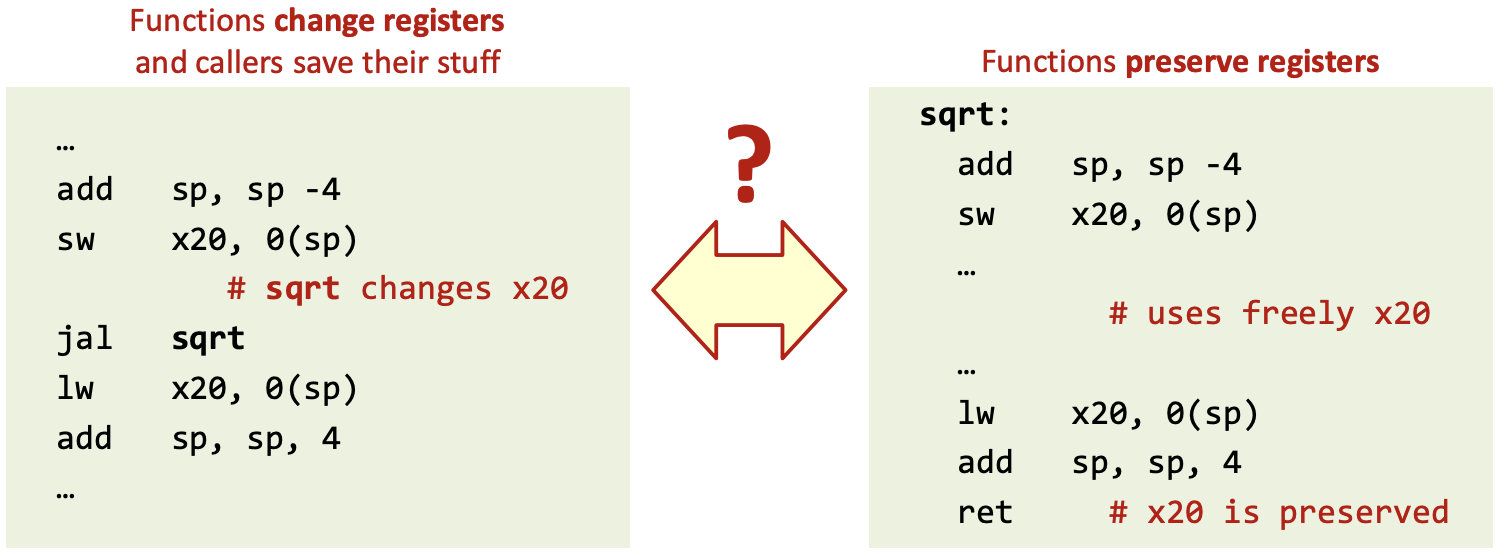
\includegraphics[width=0.7\textwidth]{chapters/chapter1b/images/registers.png}
\end{center}

\subsection{Preserving Registers}
In RISC-V, register preservation is managed through a combination of callee-saved and caller-saved registers. \\
Callee-saved registers (such as \texttt{s0}, \texttt{s1}, and \texttt{s2-11}) are preserved by the called function, ensuring that their values remain unchanged after the function call.  \\
Caller-saved registers (such as \texttt{t0}, \texttt{t1-2}, and \texttt{t3-6}) are temporary and do not need to be preserved by the called function, meaning the caller must save them if their values are important. \\
\begin{center}
    \begin{tabular}{|c|c|c|c|}
        \hline
        \textbf{Register} & \textbf{ABI Name} & \textbf{Description} & \textbf{Preserved across call?} \\ \hline
        x0  & zero  & Hard-wired zero                        & \textemdash    \\ \hline
        x1  & ra    & Return address                         & No             \\ \hline
        x2  & sp    & Stack pointer                          & Yes            \\ \hline
        x5  & t0    & Temporary/alternate link register      & No             \\ \hline
        x6--7 & t1--2 & Temporaries                          & No             \\ \hline
        x8  & s0/fp & Saved register/frame pointer           & Yes            \\ \hline
        x9  & s1    & Saved register                        & Yes            \\ \hline
        x18--27 & s2--11 & Saved registers                   & Yes            \\ \hline
        x28--31 & t3--6 & Temporaries                        & No             \\ \hline
        \end{tabular}
\end{center}

\section{Passing Arguments in RISC-V}

In RISC-V, there are two main ways to pass arguments to functions:

\subsection{Option 1: Using Registers}
- Specific registers are used to pass arguments and return results. \\
\vskip 0.1in
- This can be done in a straightforward way, where each function uses different registers (e.g., passing an argument in \texttt{x5} and returning the result in \texttt{x6}).
\vskip 0.1in
- A more structured approach is to follow a convention where arguments are passed in registers \texttt{x10} to \texttt{x17}, with results returned in \texttt{x10}.  \\
\vskip 0.1in
- The limitation: if there are more arguments than available registers (e.g., more than 8 arguments), this approach is insufficient.  \\

\subsection{Option 2: Using the Stack}
- When registers are not enough, extra arguments are placed on the stack.  \\
\vskip 0.1in
- The stack offers a universal solution because it has no practical limit on size.  \\
\vskip 0.1in
- However, using the stack is more complex and requires additional work compared to using registers.  \\

\subsection{The RISC-V Approach}
- RISC-V uses a combination of both methods.  \\
\vskip 0.1in
- Registers \texttt{x10} to \texttt{x17} are used to pass arguments, with \texttt{x10} and \texttt{x11} also handling return values. \\
\vskip 0.1in
- If more arguments are needed beyond what these registers can handle, they are passed via the stack. 

\begin{center}
    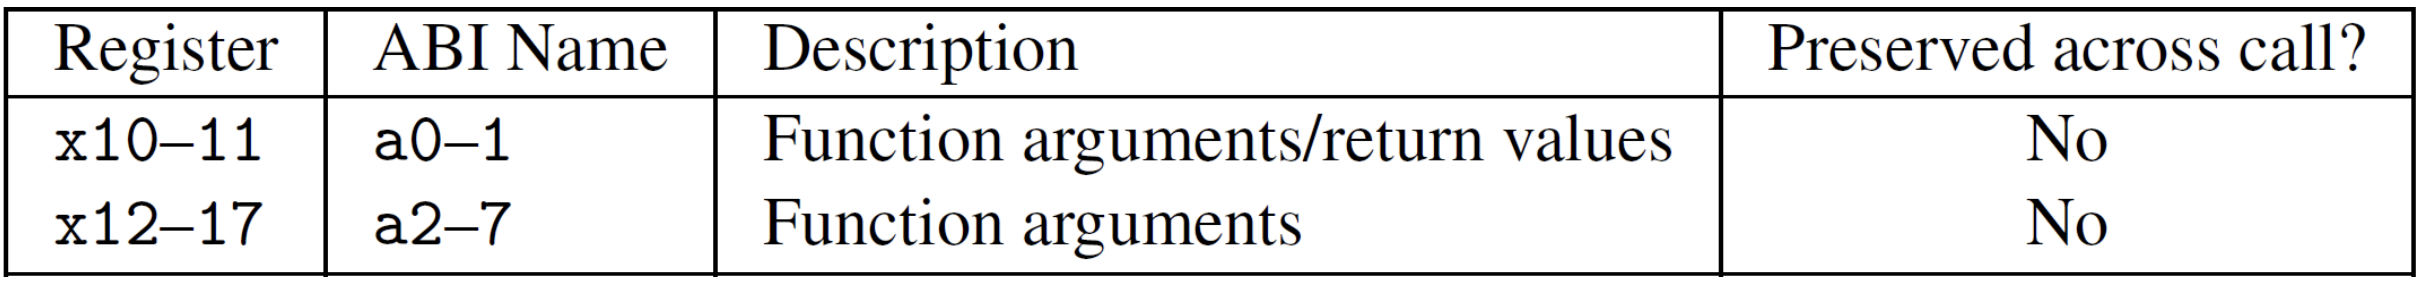
\includegraphics[width=0.75\textwidth]{chapters/chapter1b/images/arguments.png}
\end{center}
\textit{Register reserved for arguments and return values in RISC-V.}

\section{Summary of RISC-V Register Conventions}
\begin{center}
    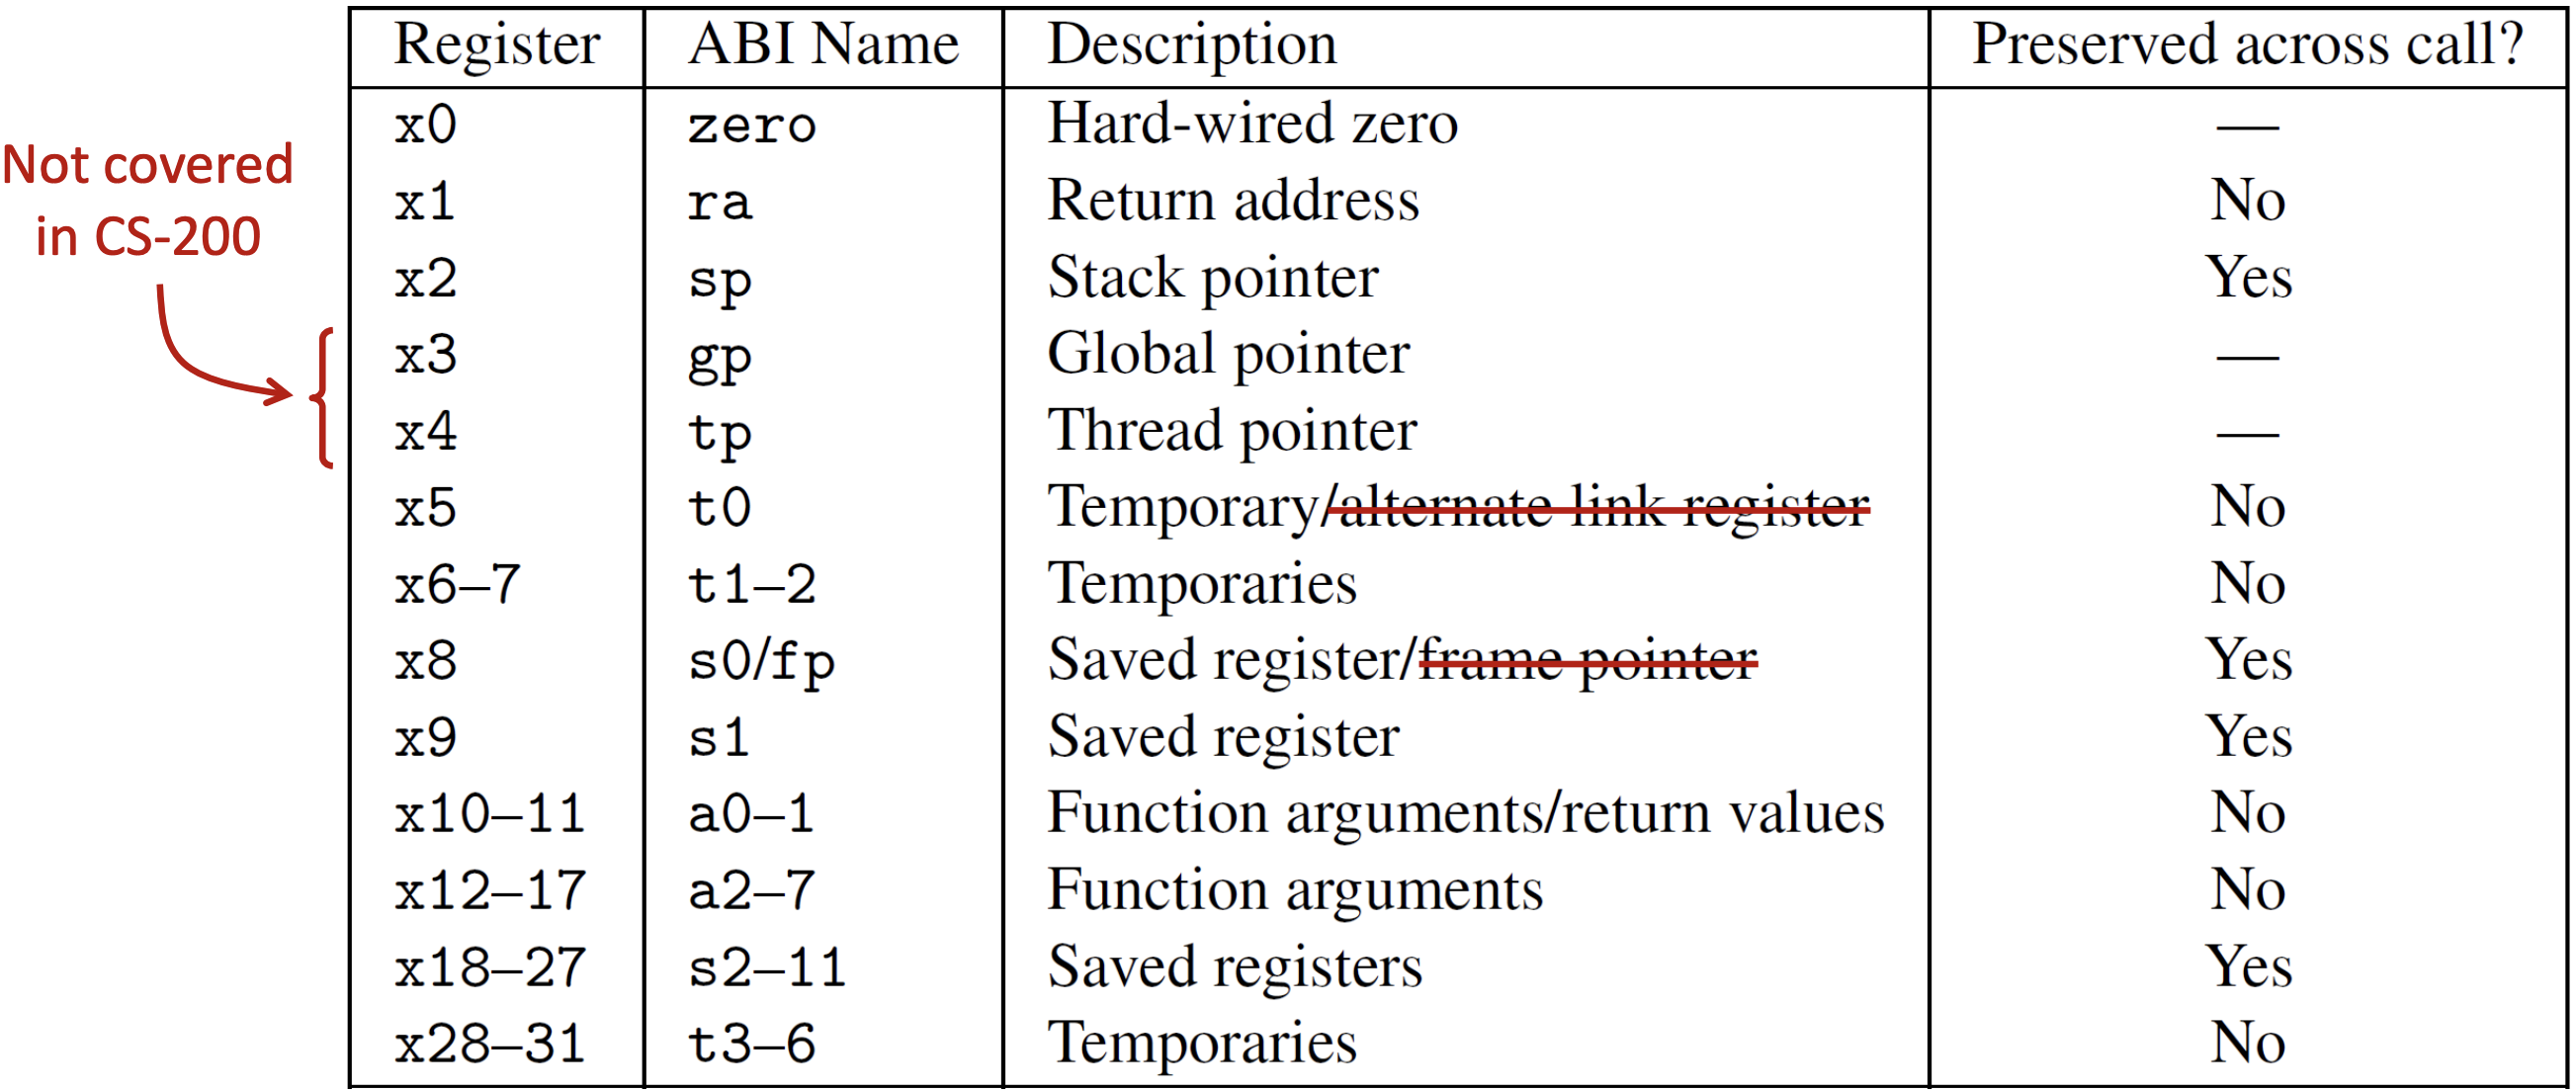
\includegraphics[width=0.75\textwidth]{chapters/chapter1b/images/summary.png}
\end{center}